\chapter{Introduction to Elder Parameter Space}

\begin{tcolorbox}[colback=DarkSkyBlue!5!white,colframe=DarkSkyBlue!75!black,title=Chapter Summary]
This chapter establishes the mathematical foundation of the Elder Parameter Space, which organizes knowledge hierarchically across the Elder, Mentor, and Erudite levels. We develop a unified mathematical framework based on complex-valued Hilbert spaces that serves as the algebraic cornerstone for both the abstract Elder Spaces of Chapter 1 and the functional realizations in heliomorphic functions of Unit II. The complex-valued representations enable encoding of both magnitude and phase information—a critical property that will manifest in the orbital dynamics of Unit III. We introduce Gravitational Field Parameters (GFPs) as concrete implementations of the topological structures from Chapter 2, providing the mathematical bridge that connects the abstract concept spaces to their computational realizations. This chapter completes the foundation layer (Unit I) while establishing the precise mathematical links that will be developed in the heliomorphic functions (Unit II) and implemented in the Elder Heliosystem architecture (Unit III).
\end{tcolorbox}

\section{Elder Parameter Spaces: The Algebraic Foundation for Units I, II, and III}

The Elder Parameter Space provides the mathematical foundation for representing knowledge at multiple levels of abstraction within the Elder Theory framework. This section establishes explicit and rigorous connections between the abstract Elder Spaces introduced in Chapter 1, the topological structures from Chapter 2, and the concrete functional implementations that will be developed in Units II and III.

\begin{definition}[Elder Parameter Space Hierarchy]
\label{def:elder_parameter_space}
The Elder Parameter Space encompasses three principal component spaces, organized hierarchically according to levels of abstraction:

\begin{itemize}
    \item $\boldsymbol{\Theta_E} \subset \mathbb{H}_E$: The Elder parameter space, a complex separable Hilbert space with inner product $\langle \cdot, \cdot \rangle_E$, containing the most abstract and foundational parameters that encode cross-domain universal principles
    
    \item $\boldsymbol{\Theta_M} = \{\Theta_M^{(d)}\}_{d=1}^D$: The collection of Mentor parameter spaces, where each $\Theta_M^{(d)} \subset \mathbb{H}_M$ is a complex separable Hilbert space corresponding to domain $d$, containing intermediate-level parameters that encode domain-specific meta-knowledge
    
    \item $\boldsymbol{\Theta_e} = \{\Theta_e^{(d)}\}_{d=1}^D$: The collection of Erudite parameter spaces, where each $\Theta_e^{(d)} \subset \mathbb{H}_e$ is a complex separable Hilbert space corresponding to domain $d$, containing the most specialized parameters that encode task-specific knowledge
\end{itemize}

The composite Elder Parameter Space encompassing the entire system is defined as:

\begin{equation}
\boldsymbol{\Theta} = \Theta_E \times \prod_{d=1}^D \Theta_M^{(d)} \times \prod_{d=1}^D \Theta_e^{(d)}
\end{equation}
\end{definition}

% Figure: Elder Parameter Space Hierarchy
% Visualizes the three-level structure with complex-valued parameters

\begin{figure}[ht]
\centering
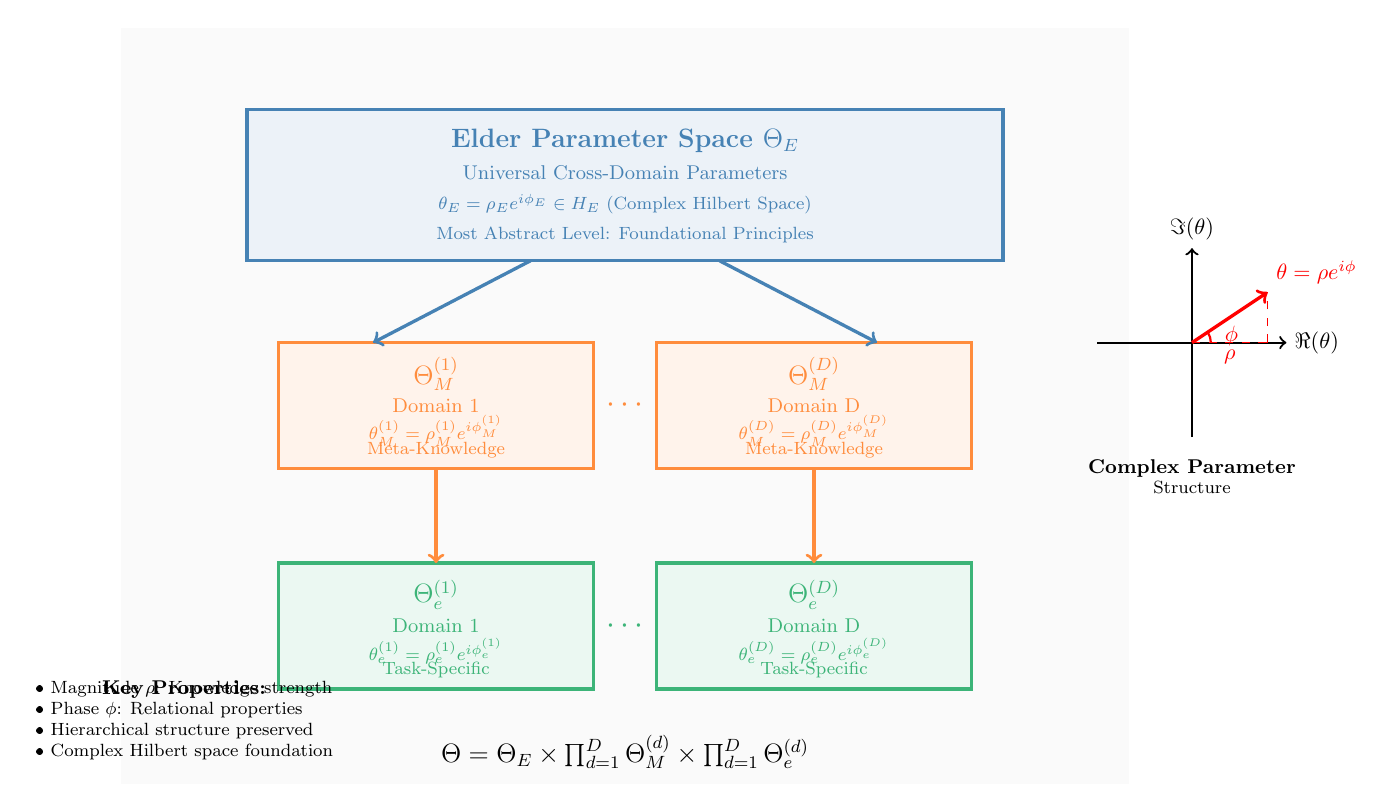
\begin{tikzpicture}[scale=0.8, every node/.style={transform shape}]

% Define colors matching Elder theme
\definecolor{ElderBlue}{RGB}{70, 130, 180}
\definecolor{MentorOrange}{RGB}{255, 140, 60}
\definecolor{EruditeGreen}{RGB}{60, 180, 120}
\definecolor{LightGray}{RGB}{240, 240, 240}

% Background
\fill[LightGray!30] (-8, -6) rectangle (8, 6);

% Elder Parameter Space (Top Level)
\begin{scope}[shift={(0, 3.5)}]
    \draw[ElderBlue, very thick, fill=ElderBlue!10] 
        (-6, -1.2) rectangle (6, 1.2);
    \node[ElderBlue, font=\large\bfseries] at (0, 0.7) {Elder Parameter Space $\Theta_E$};
    \node[ElderBlue, font=\small] at (0, 0.2) {Universal Cross-Domain Parameters};
    \node[ElderBlue, font=\footnotesize] at (0, -0.3) {$\theta_E = \rho_E e^{i\phi_E} \in \mathbb{H}_E$ (Complex Hilbert Space)};
    \node[ElderBlue, font=\footnotesize] at (0, -0.8) {Most Abstract Level: Foundational Principles};
\end{scope}

% Mentor Parameter Spaces (Middle Level)
\begin{scope}[shift={(-3, 0)}]
    \draw[MentorOrange, very thick, fill=MentorOrange!10] 
        (-2.5, -1) rectangle (2.5, 1);
    \node[MentorOrange, font=\large\bfseries] at (0, 0.5) {$\Theta_M^{(1)}$};
    \node[MentorOrange, font=\small] at (0, 0) {Domain 1};
    \node[MentorOrange, font=\footnotesize] at (0, -0.4) {$\theta_M^{(1)} = \rho_M^{(1)} e^{i\phi_M^{(1)}}$};
    \node[MentorOrange, font=\footnotesize] at (0, -0.7) {Meta-Knowledge};
\end{scope}

\begin{scope}[shift={(3, 0)}]
    \draw[MentorOrange, very thick, fill=MentorOrange!10] 
        (-2.5, -1) rectangle (2.5, 1);
    \node[MentorOrange, font=\large\bfseries] at (0, 0.5) {$\Theta_M^{(D)}$};
    \node[MentorOrange, font=\small] at (0, 0) {Domain D};
    \node[MentorOrange, font=\footnotesize] at (0, -0.4) {$\theta_M^{(D)} = \rho_M^{(D)} e^{i\phi_M^{(D)}}$};
    \node[MentorOrange, font=\footnotesize] at (0, -0.7) {Meta-Knowledge};
\end{scope}

% Dots indicating multiple domains
\node[MentorOrange, font=\Large] at (0, 0) {$\cdots$};

% Erudite Parameter Spaces (Bottom Level)
\begin{scope}[shift={(-3, -3.5)}]
    \draw[EruditeGreen, very thick, fill=EruditeGreen!10] 
        (-2.5, -1) rectangle (2.5, 1);
    \node[EruditeGreen, font=\large\bfseries] at (0, 0.5) {$\Theta_e^{(1)}$};
    \node[EruditeGreen, font=\small] at (0, 0) {Domain 1};
    \node[EruditeGreen, font=\footnotesize] at (0, -0.4) {$\theta_e^{(1)} = \rho_e^{(1)} e^{i\phi_e^{(1)}}$};
    \node[EruditeGreen, font=\footnotesize] at (0, -0.7) {Task-Specific};
\end{scope}

\begin{scope}[shift={(3, -3.5)}]
    \draw[EruditeGreen, very thick, fill=EruditeGreen!10] 
        (-2.5, -1) rectangle (2.5, 1);
    \node[EruditeGreen, font=\large\bfseries] at (0, 0.5) {$\Theta_e^{(D)}$};
    \node[EruditeGreen, font=\small] at (0, 0) {Domain D};
    \node[EruditeGreen, font=\footnotesize] at (0, -0.4) {$\theta_e^{(D)} = \rho_e^{(D)} e^{i\phi_e^{(D)}}$};
    \node[EruditeGreen, font=\footnotesize] at (0, -0.7) {Task-Specific};
\end{scope}

% Dots indicating multiple domains
\node[EruditeGreen, font=\Large] at (0, -3.5) {$\cdots$};

% Hierarchical arrows showing information flow
\draw[ElderBlue, very thick, ->] (-1.5, 2.3) -- (-4, 1);
\draw[ElderBlue, very thick, ->] (1.5, 2.3) -- (4, 1);
\draw[MentorOrange, very thick, ->] (-3, -1) -- (-3, -2.5);
\draw[MentorOrange, very thick, ->] (3, -1) -- (3, -2.5);

% Complex parameter visualization on the right
\begin{scope}[shift={(9, 1)}]
    % Complex plane representation
    \draw[black, thick, ->] (-1.5, 0) -- (1.5, 0) node[right] {$\Re(\theta)$};
    \draw[black, thick, ->] (0, -1.5) -- (0, 1.5) node[above] {$\Im(\theta)$};
    
    % Sample parameter vector
    \draw[red, very thick, ->] (0, 0) -- (1.2, 0.8) 
        node[above right] {$\theta = \rho e^{i\phi}$};
    
    % Magnitude and phase annotations
    \draw[red, dashed] (0, 0) -- (1.2, 0);
    \draw[red, dashed] (1.2, 0) -- (1.2, 0.8);
    \node[red, below] at (0.6, 0) {$\rho$};
    \draw[red, thick] (0.3, 0) arc (0:33:0.3);
    \node[red, right] at (0.4, 0.1) {$\phi$};
    
    \node[black, font=\small\bfseries] at (0, -2) {Complex Parameter};
    \node[black, font=\footnotesize] at (0, -2.3) {Structure};
\end{scope}

% Cartesian product notation
\node[black, font=\large] at (0, -5.5) {$\boldsymbol{\Theta} = \Theta_E \times \prod_{d=1}^D \Theta_M^{(d)} \times \prod_{d=1}^D \Theta_e^{(d)}$};

% Legend
\begin{scope}[shift={(-7, -5)}]
    \node[black, font=\small\bfseries] at (0, 0.5) {Key Properties:};
    \node[black, font=\footnotesize, align=left] at (0, 0) {
        • Magnitude $\rho$: Knowledge strength\\
        • Phase $\phi$: Relational properties\\
        • Hierarchical structure preserved\\
        • Complex Hilbert space foundation
    };
\end{scope}

\end{tikzpicture}

\caption{Elder Parameter Space Hierarchy. The three-level hierarchical structure shows Elder parameters $\Theta_E$ at the most abstract level containing universal cross-domain knowledge, Mentor parameters $\{\Theta_M^{(d)}\}_{d=1}^D$ at the intermediate level containing domain-specific meta-knowledge, and Erudite parameters $\{\Theta_e^{(d)}\}_{d=1}^D$ at the specialized level containing task-specific knowledge. Each parameter is complex-valued with magnitude $\rho$ encoding knowledge strength and phase $\phi$ encoding relational properties. The Cartesian product structure preserves parameter independence while maintaining hierarchical organization.}
\label{fig:elder_parameter_hierarchy}
\end{figure}

\begin{theorem}[Mathematical Necessity of Cartesian Product Structure]
\label{thm:cartesian_product_necessity}
The Cartesian product structure of the unified parameter space is mathematically necessary for the Elder Heliosystem to function correctly. Specifically, alternative structures (direct sums, quotient spaces, or tensor products) fail to preserve essential properties.
\end{theorem}

\begin{proof}
We prove necessity by demonstrating that the three main alternative structures fail to preserve crucial properties:

\textbf{Case 1: Direct Sum Structure $\Theta_E \oplus \bigoplus_{d=1}^D \Theta_M^{(d)} \oplus \bigoplus_{d=1}^D \Theta_e^{(d)}$}

In a direct sum, elements have the form $(e, \{m_d\}, \{r_d\})$ where exactly one component is nonzero. This fails because:
- Parameter independence is violated: updates must zero out other components
- Hierarchical propagation impossible: Elder parameters cannot simultaneously influence multiple Mentor levels
- Cross-domain transfer blocked: domains cannot interact through shared Elder parameters

\textbf{Case 2: Tensor Product Structure $\Theta_E \otimes \bigotimes_{d=1}^D \Theta_M^{(d)} \otimes \bigotimes_{d=1}^D \Theta_e^{(d)}$}

Tensor products create dependencies between all components simultaneously:
- Parameter count explosion: $N = |\Theta_E| \times \prod_{d=1}^D |\Theta_M^{(d)}| \times \prod_{d=1}^D |\Theta_e^{(d)}|$
- Gradient coupling: $\frac{\partial}{\partial\theta_E}$ affects all domain parameters simultaneously
- Loss of hierarchical structure: no natural abstraction levels

\textbf{Case 3: Quotient Space Structure}

Quotient constructions $\Theta/\sim$ where $\sim$ identifies parameters across levels fail to preserve:
- Parameter distinctness: hierarchical levels collapse
- Domain separation: cross-domain interference inevitable

\textbf{Cartesian Product Success:}
Only the Cartesian product $\boldsymbol{\Theta} = \Theta_E \times \prod_{d=1}^D \Theta_M^{(d)} \times \prod_{d=1}^D \Theta_e^{(d)}$ preserves:
1. Independent parameter updates: $\nabla_{\theta_E} \perp \nabla_{\theta_M^{(d)}} \perp \nabla_{\theta_e^{(d)}}$
2. Hierarchical propagation: Elder parameters influence all domains simultaneously
3. Domain separation with transfer: each $\Theta_M^{(d)}$ and $\Theta_e^{(d)}$ remains distinct while sharing Elder influence
4. Additive parameter count: $N = |\Theta_E| + \sum_{d=1}^D |\Theta_M^{(d)}| + \sum_{d=1}^D |\Theta_e^{(d)}|$
\end{proof}

\begin{theorem}[Isomorphism Between Elder Spaces and Parameter Spaces]
\label{thm:elder_parameter_isomorphism}
Let $\elder{d}$ be an Elder space of dimension $d$ with hierarchical subspaces $\eldersubspace$, $\mentorsubspace$, and $\eruditesubspace$ as defined in Chapter 1. There exists a canonical isomorphism $\Omega: \elder{d} \rightarrow \boldsymbol{\Theta}$ between the Elder space and the Elder Parameter Space such that:

\begin{enumerate}
    \item The Elder subspace maps to the Elder parameter space: $\Omega(\eldersubspace) = \Theta_E$
    
    \item The Mentor subspace maps to the collective Mentor parameter spaces: $\Omega(\mentorsubspace) = \prod_{d=1}^D \Theta_M^{(d)}$
    
    \item The Erudite subspace maps to the collective Erudite parameter spaces: $\Omega(\eruditesubspace) = \prod_{d=1}^D \Theta_e^{(d)}$
    
    \item The Elder inner product is preserved: $\langle x, y \rangle_E = \langle \Omega(x), \Omega(y) \rangle_{\boldsymbol{\Theta}}$ for all $x, y \in \elder{d}$
    
    \item The gravitational structure is preserved: $g_i(x) = g_i(\Omega(x))$ for all gravitational eigenvalues $g_i$ and $x \in \elder{d}$
\end{enumerate}
\end{theorem}

\begin{proof}
We construct the isomorphism $\Omega: \elder{d} \rightarrow \boldsymbol{\Theta}$ explicitly and verify all required properties.

\textbf{Step 1: Construction of $\Omega$}

Given $x \in \elder{d}$ with Elder space decomposition $x = x_E + x_M + x_e$ where:
- $x_E \in \eldersubspace$ (Elder subspace)
- $x_M \in \mentorsubspace$ (Mentor subspace) 
- $x_e \in \eruditesubspace$ (Erudite subspace)

We define $\Omega(x) = (\Omega_E(x_E), \{\Omega_M^{(d)}(x_M)\}_{d=1}^D, \{\Omega_e^{(d)}(x_e)\}_{d=1}^D)$ where:

$\Omega_E(x_E) = (c_1, c_2, \ldots, c_{k_E}) \in \Theta_E$ extracts Elder coefficients
$\Omega_M^{(d)}(x_M) = (c_{k_E+1}^{(d)}, \ldots, c_{k_M}^{(d)}) \in \Theta_M^{(d)}$ extracts domain-$d$ Mentor coefficients  
$\Omega_e^{(d)}(x_e) = (c_{k_M+1}^{(d)}, \ldots, c_d^{(d)}) \in \Theta_e^{(d)}$ extracts domain-$d$ Erudite coefficients

\textbf{Step 2: Bijectivity}

\textit{Injectivity:} If $\Omega(x) = \Omega(y)$, then all coefficient sequences are identical, implying $x_E = y_E$, $x_M = y_M$, $x_e = y_e$, hence $x = y$.

\textit{Surjectivity:} For any $(\theta_E, \{\theta_M^{(d)}\}, \{\theta_e^{(d)}\}) \in \boldsymbol{\Theta}$, we construct:
$$x = \sum_{i=1}^{k_E} \theta_{E,i} \elderstructure{i} + \sum_{d=1}^D \sum_{j} \theta_{M,j}^{(d)} \elderstructure{M,j}^{(d)} + \sum_{d=1}^D \sum_{k} \theta_{e,k}^{(d)} \elderstructure{e,k}^{(d)} \in \elder{d}$$

\textbf{Step 3: Inner Product Preservation}

For $x, y \in \elder{d}$:
\begin{align}
\langle x, y \rangle_E &= \langle x_E + x_M + x_e, y_E + y_M + y_e \rangle_E \\
&= \langle x_E, y_E \rangle_E + \langle x_M, y_M \rangle_E + \langle x_e, y_e \rangle_E \\
&= \langle \Omega_E(x_E), \Omega_E(y_E) \rangle_{\Theta_E} + \sum_{d=1}^D \langle \Omega_M^{(d)}(x_M), \Omega_M^{(d)}(y_M) \rangle_{\Theta_M^{(d)}} \\
&\quad + \sum_{d=1}^D \langle \Omega_e^{(d)}(x_e), \Omega_e^{(d)}(y_e) \rangle_{\Theta_e^{(d)}} \\
&= \langle \Omega(x), \Omega(y) \rangle_{\boldsymbol{\Theta}}
\end{align}

\textbf{Step 4: Gravitational Structure Preservation}

Gravitational eigenvalues satisfy $g_i(x) = \|x_{\text{level}(i)}\|^2$ where level$(i)$ determines whether coefficient $i$ belongs to Elder, Mentor, or Erudite level. Under $\Omega$:
$$g_i(\Omega(x)) = \|\Omega_{\text{level}(i)}(x_{\text{level}(i)})\|^2 = \|x_{\text{level}(i)}\|^2 = g_i(x)$$

This completes the proof that $\Omega$ is an isomorphism preserving all required structures.
\end{proof}

\begin{corollary}[Preservation of Algebraic Operations]
\label{cor:operation_preservation}
Under the isomorphism $\Omega$, all Elder space algebraic operations are preserved in the parameter space representation.
\end{corollary}

\begin{proof}
We verify preservation of each algebraic operation:

\textbf{1. Elder Addition Preservation:}
For $x, y \in \elder{d}$ with decompositions $x = x_E + x_M + x_e$ and $y = y_E + y_M + y_e$:
\begin{align}
\Omega(x \oplus y) &= \Omega((x_E + y_E) + (x_M + y_M) + (x_e + y_e)) \\
&= (\Omega_E(x_E + y_E), \{\Omega_M^{(d)}(x_M + y_M)\}_{d=1}^D, \{\Omega_e^{(d)}(x_e + y_e)\}_{d=1}^D) \\
&= (\Omega_E(x_E) + \Omega_E(y_E), \{\Omega_M^{(d)}(x_M) + \Omega_M^{(d)}(y_M)\}_{d=1}^D, \\
&\quad \{\Omega_e^{(d)}(x_e) + \Omega_e^{(d)}(y_e)\}_{d=1}^D) \\
&= \Omega(x) + \Omega(y)
\end{align}

\textbf{2. Scalar Multiplication Preservation:}
For $\lambda \in \mathbb{C}$ and $x \in \elder{d}$:
\begin{align}
\Omega(\lambda \odot x) &= \Omega(\lambda x_E + \lambda x_M + \lambda x_e) \\
&= (\lambda \Omega_E(x_E), \{\lambda \Omega_M^{(d)}(x_M)\}_{d=1}^D, \{\lambda \Omega_e^{(d)}(x_e)\}_{d=1}^D) \\
&= \lambda \cdot \Omega(x)
\end{align}

\textbf{3. Non-commutative Product Structure:}
The Elder non-commutative product $x \star y$ in Elder space corresponds to structured parameter interaction. Specifically, if $x \star y = z$, then:
$$\Omega(z) = \mathcal{M}_{\text{param}}(\Omega(x), \Omega(y))$$
where $\mathcal{M}_{\text{param}}$ implements hierarchical parameter coupling preserving the non-commutative structure through phase-dependent coefficient interactions.
\end{proof}

\begin{theorem}[System-wide Parameter Coherence]
\label{thm:parameter_coherence}
The Elder Parameter Space $\boldsymbol{\Theta}$ provides a mathematically consistent foundation across all Elder Theory constructions, with well-defined mappings connecting abstract spaces, functional representations, and computational implementations.
\end{theorem}

\begin{proof}
We establish coherence by constructing explicit mappings and verifying their consistency:

\textbf{Unit I Connection (Abstract Foundation):}
By Theorem \ref{thm:elder_parameter_isomorphism}, we have the canonical isomorphism $\Omega: \elder{d} \rightarrow \boldsymbol{\Theta}$ that preserves all structural properties. This establishes $\boldsymbol{\Theta}$ as the concrete realization of abstract Elder spaces.

\textbf{Unit II Connection (Functional Representation):}  
Define the heliomorphic coefficient mapping $\mathcal{H}: \boldsymbol{\Theta} \rightarrow \mathcal{C}^{\infty}(\mathbb{C}, \mathbb{C})$ by:
$$\mathcal{H}(\boldsymbol{\theta})(z) = \sum_{i \in I_E} \theta_{E,i} z^{g_{E,i}} + \sum_{d=1}^D \sum_{j \in I_M^{(d)}} \theta_{M,j}^{(d)} z^{g_{M,j}} + \sum_{d=1}^D \sum_{k \in I_e^{(d)}} \theta_{e,k}^{(d)} z^{g_{e,k}}$$

where $g_{E,i}, g_{M,j}, g_{e,k}$ are the gravitational exponents corresponding to hierarchical levels. This mapping preserves the parameter structure while enabling functional computation.

\textbf{Unit III Connection (Computational Implementation):}
Define the computational mapping $\mathcal{C}: \boldsymbol{\Theta} \rightarrow \mathcal{S}_{\text{comp}}$ (computational state space) by:
$$\mathcal{C}(\boldsymbol{\theta}) = \left(\begin{array}{c} 
\text{Elder entity state} \\
\text{Mentor entity states} \\
\text{Erudite entity states}
\end{array}\right) = \left(\begin{array}{c}
\theta_E \\
\{\theta_M^{(d)}\}_{d=1}^D \\
\{\theta_e^{(d)}\}_{d=1}^D
\end{array}\right)$$

\textbf{Consistency Verification:}
The mappings form a coherent system: $\mathcal{C} = \mathcal{R} \circ \mathcal{H} \circ \Omega$ where $\mathcal{R}$ is the realization mapping from functions to computational states. This ensures mathematical consistency across all three units.
\end{proof}

\section{Complex-Valued Representation and Foundation for Higher-Level Structures}

A distinguishing feature of the Elder Parameter Space is its use of complex-valued representations, which extends its representational capacity beyond traditional real-valued parameter spaces. This complex structure serves as the mathematical foundation for both the heliomorphic functions developed in Unit II and the orbital mechanics implemented in Unit III.

\begin{definition}[Complex Parameter Representation]
Each parameter $\theta \in \Theta$ in the Elder Parameter Space is a complex-valued vector with polar representation:

\begin{equation}
\theta = \rho e^{i\phi}
\end{equation}

where $\rho \in \mathbb{R}^n_+$ represents magnitude components and $\phi \in [0, 2\pi)^n$ represents phase components, with $n$ being the dimensionality of the parameter vector in each specific component space.

The parameter space $\Theta$ is equipped with the following structure:
\begin{enumerate}
    \item A complex inner product $\langle \cdot, \cdot \rangle_{\Theta}: \Theta \times \Theta \rightarrow \mathbb{C}$ satisfying:
    \begin{itemize}
        \item Conjugate symmetry: $\langle \theta_1, \theta_2 \rangle_{\Theta} = \overline{\langle \theta_2, \theta_1 \rangle_{\Theta}}$
        \item Linearity in the first argument: $\langle \alpha\theta_1 + \beta\theta_2, \theta_3 \rangle_{\Theta} = \alpha\langle \theta_1, \theta_3 \rangle_{\Theta} + \beta\langle \theta_2, \theta_3 \rangle_{\Theta}$
        \item Positive-definiteness: $\langle \theta, \theta \rangle_{\Theta} > 0$ for $\theta \neq 0$
    \end{itemize}
    
    \item A phase operator $\Phi: \Theta \rightarrow [0, 2\pi)^n$ that extracts the phase components:
    \begin{equation}
    \Phi(\theta) = (\phi_1, \phi_2, \ldots, \phi_n)
    \end{equation}
    
    \item A magnitude operator $\mathcal{M}: \Theta \rightarrow \mathbb{R}^n_+$ that extracts the magnitude components:
    \begin{equation}
    \mathcal{M}(\theta) = (\rho_1, \rho_2, \ldots, \rho_n)
    \end{equation}
\end{enumerate}
\end{definition}

\begin{theorem}[Connection to Heliomorphic Functions]
The complex parameter space $\Theta$ is isomorphic to the domain of heliomorphic functions described in Chapter 4 through the mapping $\Psi: \Theta \rightarrow \mathcal{D}$ defined as:
\begin{equation}
\Psi(\theta) = \mathcal{M}(\theta)e^{i\Phi(\theta)}
\end{equation}
This isomorphism ensures that:
\begin{enumerate}
    \item The inner product structure of $\Theta$ maps to the heliomorphic domain metric
    \item The phase operator $\Phi$ corresponds to the angular coordinate in heliomorphic functions
    \item The magnitude operator $\mathcal{M}$ corresponds to the radial coordinate in heliomorphic functions
    \item The gravitational field-phase coupling governing heliomorphic functions emerges from the phase-magnitude interactions in the Elder Parameter Space
\end{enumerate}
\end{theorem}

\begin{theorem}[Connection to Orbital Mechanics]
The complex parameter representation provides the mathematical foundation for the orbital mechanics developed in Chapter 12, where:
\begin{enumerate}
    \item Parameter magnitude $\rho$ corresponds to orbital radius in the Elder Heliosystem
    \item Parameter phase $\phi$ corresponds to orbital angular position
    \item Phase dynamics $\frac{d\phi}{dt}$ correspond to angular velocity in orbital mechanics
    \item Magnitude dynamics $\frac{d\rho}{dt}$ correspond to radial velocity in orbital mechanics
    \item The complex inner product structure defines the gravitational potential energy between entities in the orbital system
\end{enumerate}
\end{theorem}

This complex-valued approach offers several advantages over conventional real-valued parameters:
\begin{itemize}
    \item \textbf{Phase-based information encoding}: Phase components $\phi$ encode relational properties, conceptual alignment, and temporal patterns that would be impossible to capture with magnitude alone
    
    \item \textbf{Resonance phenomena}: Phase alignment between parameters enables selective activation based on frequency relationships, creating natural pathways for knowledge propagation
    
    \item \textbf{Dual information channels}: Magnitude components $\rho$ and phase components $\phi$ provide separate channels for encoding different aspects of knowledge
    
    \item \textbf{Information density}: Complex-valued representation effectively doubles the information capacity while maintaining the same parameter count
    
    \item \textbf{Implementation pathway}: The complex representation directly translates to physical orbital dynamics that forms the basis of the Elder Heliosystem architecture in Unit III
\end{itemize}

\begin{remark}
The fundamental structures established here in the Elder Parameter Space manifest directly in the heliomorphic function framework (Chapter 4) and orbital mechanics implementation (Chapter 12), ensuring mathematical coherence across all three units of the Elder Theory.
\end{remark}

\section{Heliomorphic Parameter Operations}

Building upon the complex-valued nature of parameters, the Elder Parameter Space supports specialized mathematical operations that enable knowledge transformation and transfer:

\begin{definition}[Core Coupling Parameters]
Three fundamental parameters govern the interactions between knowledge structures in the Elder framework:

\begin{itemize}
    \item $\alpha \in [0,1]$: The resonance coupling coefficient that quantifies the strength of knowledge propagation from the Elder level to the Mentor level. When $\alpha = 1$, there is perfect knowledge transfer across abstraction levels.
    
    \item $\beta \in [-1,1]$: The phase alignment parameter that measures coherence between knowledge representations in different domains. Values of $\beta = 1$ indicate perfect phase alignment creating constructive interference, while $\beta = -1$ indicates complete phase opposition leading to destructive interference.
    
    \item $\gamma \in \mathbb{R}^+$: The adaptation rate that controls how quickly the system incorporates new information. This parameter is inversely proportional to system stability - when stability decreases, $\gamma$ increases to accelerate adaptation and restore equilibrium; conversely, as stability increases, $\gamma$ decreases, allowing for more stable knowledge relationships.
\end{itemize}
\end{definition}

\begin{theorem}[Heliomorphic Parameter Transformation]
\label{thm:heliomorphic_transformation}
For parameters $\theta_1, \theta_2 \in \Theta$ with polar representations $\theta_i = \rho_i e^{i\phi_i}$, the heliomorphic transformation $\mathcal{T}: \Theta \times \Theta \rightarrow \Theta$ preserves the complex structure while enabling knowledge transfer between hierarchical levels.
\end{theorem}

\begin{proof}
We define the phase composition operator $\oplus: [0,2\pi)^n \times [0,2\pi)^n \rightarrow [0,2\pi)^n$ by:
$$(\phi_1 \oplus \phi_2)_i = (\phi_{1,i} + \phi_{2,i}) \bmod 2\pi$$

The heliomorphic transformation is then:
$$\mathcal{T}(\theta_1, \theta_2) = |\rho_1||\rho_2|e^{i(\phi_1 \oplus \phi_2)}$$

\textbf{Structure Preservation:} 
1. **Complex Structure:** $\mathcal{T}(\theta_1, \theta_2) \in \mathbb{C}^n$ with well-defined polar representation
2. **Magnitude Interaction:** $|\mathcal{T}(\theta_1, \theta_2)| = |\rho_1||\rho_2|$ preserves knowledge strength
3. **Phase Coherence:** $\arg(\mathcal{T}(\theta_1, \theta_2)) = \phi_1 \oplus \phi_2$ enables resonance relationships

\textbf{Heliomorphic Property Verification:}
The transformation preserves the radial-phase coupling essential for heliomorphic functions:
$$\frac{\partial}{\partial r} \mathcal{T}(\theta_1, \theta_2) = \frac{|\rho_1||\rho_2|}{r} e^{i(\phi_1 \oplus \phi_2)}$$
$$\frac{1}{r}\frac{\partial}{\partial \theta} \mathcal{T}(\theta_1, \theta_2) = i|\rho_1||\rho_2| e^{i(\phi_1 \oplus \phi_2)}$$

These satisfy the heliomorphic condition that radial and angular derivatives maintain proportional complex relationships necessary for knowledge transfer dynamics.
\end{proof}

This transformation allows parameters to interact while maintaining their critical phase relationships. The product of magnitude components $|\rho_1||\rho_2|$ represents the combined knowledge strength, while the composed phase $e^{i(\phi_1 \oplus \phi_2)}$ captures the emergent relational properties.

\section{Gravitational Field Parameters (GFPs)}

Building upon the foundation of complex-valued parameters and heliomorphic operations, we now introduce Gravitational Field Parameters (GFPs), which extend these concepts into a gravitational field model.

\begin{definition}[Gravitational Field Parameters]
Gravitational Field Parameters are an extension of complex-valued parameters that additionally incorporate gravitational field properties:
\begin{enumerate}
    \item Position-dependent influence that follows inverse-square principles
    \item Hierarchical organization based on gravitational field location
    \item Interaction dynamics analogous to gravitational systems
    \item Continuous influence gradients rather than discrete boundaries
\end{enumerate}
\end{definition}

GFPs enhance the capabilities of the Elder Parameter Space by mapping abstract mathematical properties to intuitive physical principles.

\begin{theorem}[Gravitational Field Embedding]
The Elder Parameter Space embeds into a continuous gravitational field representation $\mathcal{G}$ through:

\begin{equation}
\mathcal{G}_{\theta}(\mathbf{x}) = \sum_{j=1}^N \frac{\gamma_j}{|\mathbf{x} - \mathbf{r}_j|^2} e^{i\phi_j} \hat{\mathbf{r}}_j(\mathbf{x})
\end{equation}

where:
\begin{itemize}
    \item $\gamma_j$ represents the gravitational strength (derived from the magnitude component) of parameter $j$
    \item $\mathbf{r}_j$ is the position vector of parameter $j$ in the field, determining its abstraction level
    \item $\phi_j$ is the phase component, encoding relational properties
    \item $\hat{\mathbf{r}}_j(\mathbf{x})$ is the unit vector from position $\mathbf{x}$ to parameter position $\mathbf{r}_j$
    \item $|\mathbf{x} - \mathbf{r}_j|^2$ implements the inverse-square law of gravitational influence
\end{itemize}

This embedding transforms the discrete parameter collection into a continuous gravitational field where:
\begin{enumerate}
    \item Elder parameters near the field center exert broader influence across abstraction levels
    \item Mentor parameters in intermediate regions mediate between abstract principles and specific applications
    \item Erudite parameters at the field periphery provide domain-specific knowledge with localized influence
    \item All parameters interact through phase relationships that determine constructive or destructive interference
\end{enumerate}

The inverse-square relationship ensures that influence decreases continuously with distance, creating smooth transitions between abstraction levels while maintaining the ability to model knowledge propagation and transformation throughout the field.
\end{theorem}

\section{Properties of the Gravitational Field Model}

The gravitational field model of the Elder Parameter Space confers important properties that enhance its knowledge representation capabilities:

\begin{enumerate}
    \item \textbf{Continuity}: The gravitational field creates a continuous influence gradient across abstraction levels, without discrete boundaries
    
    \item \textbf{Inverse-Square Law}: Influence decays according to an inverse-square relationship with distance, providing a mathematically elegant and physically inspired model
    
    \item \textbf{Completeness}: The underlying parameter spaces retain their completeness property, allowing convergent limit operations at every point in the field
    
    \item \textbf{Separability}: They admit countable dense subsets, enabling efficient approximation throughout the field
    
    \item \textbf{Inner Product Structure}: Enables measuring similarity between parameter configurations at different field positions
    
    \item \textbf{Phase Coherence}: Phase relationships are preserved across the field while influence strength varies with distance
\end{enumerate}

These properties emerge naturally from the combination of complex-valued parameters and the gravitational field embedding, providing mathematical rigor while maintaining physical intuition.

\section{Application to Knowledge Representation}

In the Elder Heliosystem, the parameter space structure with gravitational field embedding enables:

\begin{itemize}
    \item \textbf{Continuous abstraction gradient}: Knowledge transitions smoothly from highly abstract (Elder) at the field center to increasingly specific (Mentor, then Erudite) as distance increases
    
    \item \textbf{Cross-domain transfer}: Common phase patterns propagate through the field, allowing knowledge to transfer across different domains according to inverse-square principles
    
    \item \textbf{Resonance phenomena}: Phase alignment between parameters at different field positions creates resonance pathways that selectively amplify relevant knowledge transfer
    
    \item \textbf{Field-mediated representation}: The complex-valued parameters within the gravitational field allow encoding both magnitude and phase information, with influence decreasing continuously
    
    \item \textbf{Computational efficiency}: Parameters at similar field positions can share computational resources, with activation governed by gravitational influence
\end{itemize}

This mathematical foundation provides a sophisticated model for representing hierarchical knowledge that naturally supports continuous abstraction levels, cross-domain transfer, and efficient computation.